\begin{figure}[!htbp]
\centering
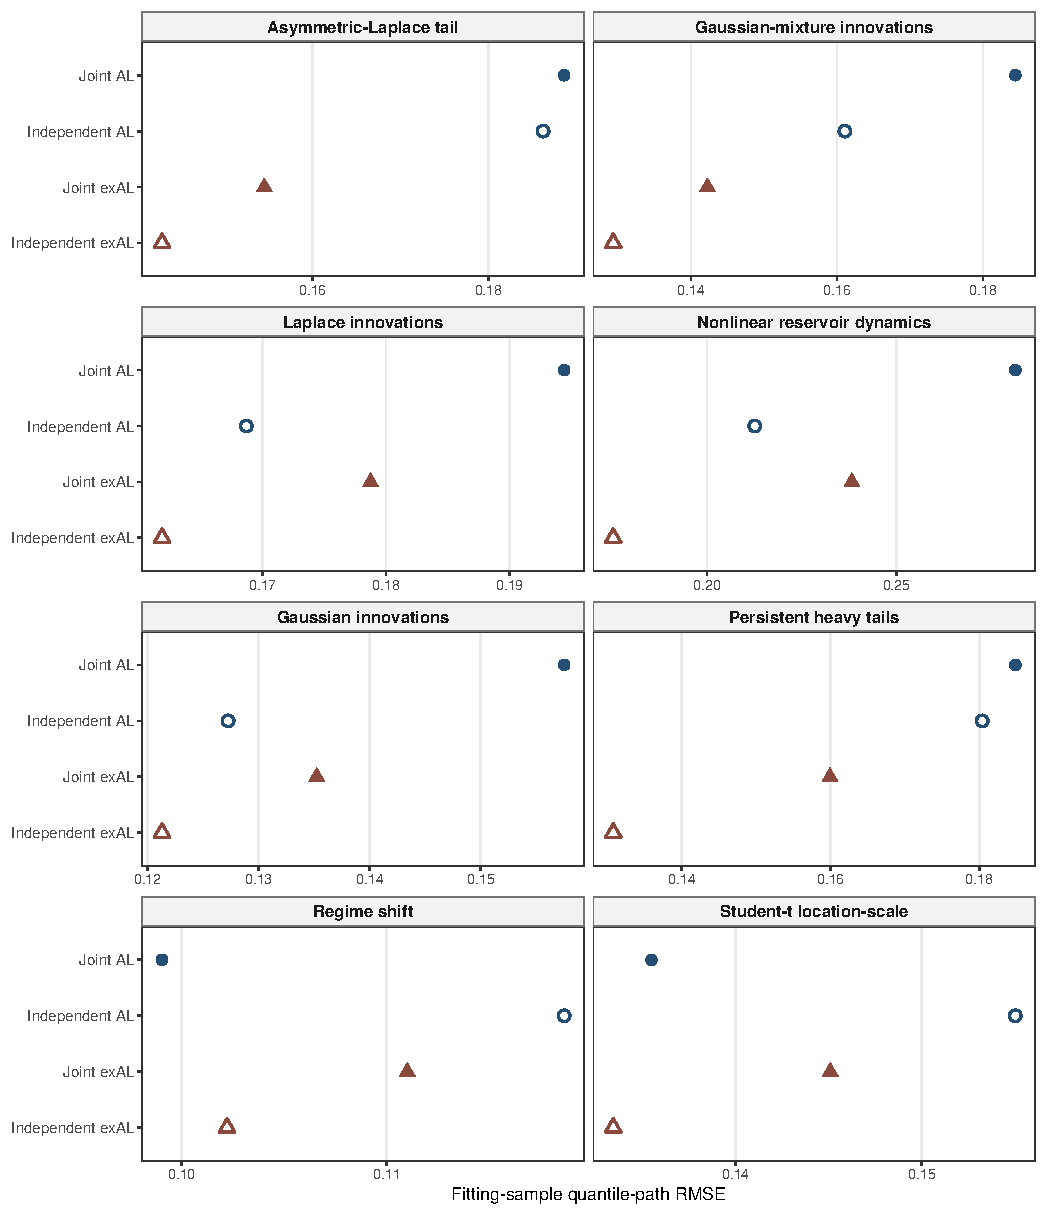
\includegraphics[width=0.94\textwidth]{figures/joint_qdesn_simulation/joint_qdesn_corrected_v4_fit_oracle_rmse.pdf}
\caption{Fitting-sample recovery of the known conditional quantile paths in the corrected joint study. Points are RMSE values for the canonical posterior-mean quantile grids, not posterior intervals. Filled symbols denote joint fits, open symbols independent fits, blue \(\AL\), and red \(\exAL\). Labels give raw/reported crossing counts; the reported grids are ordered after the pre-specified monotone rule.}
\label{fig:joint-qdesn-corrected-v4-fit-rmse}
\end{figure}
